%!TEX root = ../masters.tex

\chapter{Referencial Teórico}
\label{cha:library}

% Falar sobre RSL

% Visando obter uma revisão de literatura eficaz foi feita uma Revisão Sistemática de Literatura, com base no relatório técnico de \cite{Kitchenham}. Diante disso, o projeto se torna mais abrangente do ponto de vista de pesquisa literária e ao mesmo tempo mais restritivo, realmente realizando o estudo dos objetos que são importantes para a pesquisa e seus resultados.



% Bases pesquisadas

\begin{textedited}
Como o objetivo do trabalho tem foco na resultado prático, geralmente as bases relacionadas às áreas mais técnicas, como Ciência da Computação, devem ser bem focadas, como IEEE e ACM, por exemplo. Outras bases multidisciplinares também foram pesquisadas, através do site da CAPES, mas com caráter mais de apoio teórico.
\end{textedited}

Embora a amplitude desta área de estudo, alguns detalhes necessitam ser observados para evitar assim redundância e perda de foco. A pesquisa necessitava ser focada em técnicas de extração de metadados em artigos científicos, somente. Estas técnicas necessitam ser reais, de maneira a existir realmente uma forma prática de serem testadas, fazendo assim com que os resultados obtidos sejam comparados e confrontados para verificar então a eficácia deste processo.

\begin{textedited}
Como a pesquisa necessita de um resultado prático eficaz os critérios que serão adotados para demonstrar a relevância de um estudo serão seus resultados, sua presença de mercado e sua maturidade, visto que necessitam ainda estarem ativos para serem devidamente testados. Com base em uma técnica potencialmente eficaz, esta deve ser testada juntamente com um grupo de artigos previamente selecionados. Estes artigos já possuirão seus metadados extraídos de maneira a poder comparar os resultados obtidos com o resultado de cada uma das ferramentas. Portanto os critérios utilizados serão de natureza explicitamente prática, com foco em resultados concretos, numericamente representados.
\end{textedited}

% Falar sobre os eventos encontrados na área

\begin{textedited}
Visando abranger grande parte da literatura sobre o assunto foram mapeados alguns eventos para serem pesquisados, a fim de encontrar trabalhos relevantes para a área. Sendo assim, foram mapeados os seguintes eventos:
\end{textedited}

\begin{itemize}
    \item KDIR (International Conference of Knowledge Discovery and Information Retrieval)
    \item ICDAR (International Conference on Document Analysis and Recognition)
    \item PDCAT (International Conference on Parallel and Distributed Computing, Applications and Technologies)
    \item IAPR (International Workshop on Document Analysis Systems)
    \item ACM Conference on Digital Libraries
\end{itemize}

\begin{textedited}
Estes eventos foram analisados, observando todas as citações e referências utilizadas em cada artigo publicado, a fim de encontrar também detalhes importantes para a pesquisa, sem perder o foco do trabalho.
\end{textedited}

\section{Metadados}
\label{sec:metadados}

\comment{Esta nova seção foi incluída para definir alguns conceitos que são apresentados mais a frente com a apresentação das técnicas.}

\subsection{Conceito de Metadado}
\label{ssec:metadata-concept}

\begin{textnew}

Com base nas ideias apresentadas por \cite{meta-dados}, podemos definir inicialmente um metadado da seguinte maneira:

\begin{quote}
    \textit{''[...] an element of metadata describes an information resource, or helps provide access to an information resource.''}
\end{quote}

Sobre este aspecto conclui-se que todo dado que agregue nova informação a um recurso pode ser considerado um metadado. Desta maneira, quanto mais metadados um recurso tiver, mais detalhado ele é, ou seja, mais dados sobre ele temos. Com efeito, podemos simplificar ainda mais a definição de metadado com sendo \textit{um conjunto de dados sobre um determinado recurso}.

Temos contato diariamente com diversos metadados, sejam eles visíveis naturalmente ou não, mas de uma maneira ou outra, são utilizados em tarefas do cotidiano de maneira ampla; geralmente um conjunto enorme de novos dados e informações sobre recursos dos mais diversos tipos e modelos.

Podemos citar, por exemplo, a utilização de pequenos pedaços de dados sobre um conjunto de livros, dentro de um ambiente de biblioteca, por exemplo, o que é considerado uma coleção de elementos de metadados, conforme pode ser confirmado em \cite{meta-dados}. Além disso, o mesmo autor cita como exemplos de metadados os dados coletados por mecanismos de busca no momento em que as páginas da Internet são indexadas e então armazenadas.

Ante o exposto, podemos criar e identificar diversos conceitos do que podemos chamar de metadado, porém, em virtude de sua enorme aplicação e significância, alguns detalhes dentro do escopo deste trabalho devem ser direcionados, visando identificar e explicar melhor os conceitos que serão aplicados na análise das ferramentas e técnicas que aqui serão apresentadas.

\end{textnew}

\subsection{Padrões de Metadados}
\label{ssec:metadata-patterns}

\begin{textnew}

Diante da infinidade de dados que podem estar atrelados a um recurso, temos uma amplitude muito grande de características que podem ser definidas como sendo metadado. Por isso, foram definidos 15 (quinze) elementos de metadados para descreverem um recurso informacional, independente da disciplina em questão, estabelecendo então um padrão. 

Para isso, foi criado o padrão Dublin Core \cite{dublin-core}, que se originou após uma série de encontros feitos desde 1995, unindo bibliotecários e pesquisadores digitais e de conteúdo, visando identificar padrões para se representar um recurso eletrônico, seja ele uma página, um texto ou até mesmo um documento em um determinado formato. O nome ''Dublin'' foi dado em virtude da primeira reunião do grupo, que foi realizada em Dublin, Ohio. Já o nome ''core'' se deu em virtude dos elementos serem amplos e genéricos, sendo então utilizados para descrever uma grande variedade de recursos.

Os quinze elementos que fazem parte do padrão Dublin Core compartilham de um vasto conjunto de vocabulários de metadados, juntamente com diversas especificações técnicas, que são mantidas pela Dublin Core Metadata Initiative (DCMI), a agência responsável pela definição destes elementos.

Este padrão é utilizado nos dias atuais para se representar um recurso na Internet, por exemplo, podendo ser qualquer coisa que possa ser identificada \cite{dublin-core-1-1}. Com base em suas características, mecanismos de busca podem indexar um recurso de maneira mais rápida e precisa, pois este é acompanhado de pequenas sinalizações sobre seu conteúdo, que são os metadados. 

Para cada elemento descrito pelo padrão temos informações como: 

\begin{itemize}
    \item \textit{label}, que é o texto para leitura e entendimento humano;
    \item \textit{name}, que é usado para o processamento de máquina, ou seja, um identificador que a máquina utiliza para reconhecimento.
\end{itemize}

Os elementos que fazem parte da versão 1.1 do padrão Dublin Core \cite{dublin-core-1-1} podem ser vistos no \refanexo{attach:dublin-core} deste trabalho.

Abaixo podemos ver um exemplo de código para utilização de metadados Dublin Core em uma página da Internet, por exemplo, onde iremos referenciar os elementos \textit{creator}, \textit{title} e \textit{language}.

\lstset{language=HTML}
\begin{lstlisting}[escapechar=\#]
<meta name="DC.Creator" content="Junior Grossi" >
<meta name="DC.Title" content="#\imprimirtitulo#" >
<meta name="DC.Language" content="pt_BR" >
\end{lstlisting}

Desta forma, a indexação do autor (\textit{DC.Creator}) da página, bem como seu título (\textit{DC.Title}) e idioma (\textit{DC.Language}), são feitos de maneira bem simplificada e direta. Para páginas da Internet, com as informações todas em formato HTML, a utilização destes metadados perderiam o sentido, visto que essas informações poderiam ser facilmente encontradas de outras formas, como a análise do próprio código HTML. Porém, para documentos binários - em formato PDF ou Word, por exemplo - a utilização destes metadados é de suma importância, visto que permite que essas informações básicas sejam capturadas sem a necessidade de análise do conteúdo dos arquivos, o que traria complexidade ao processo.

\end{textnew}

\subsection{Técnicas de Extração de Metadados}
\label{ssec:metadata-techniques}

\comment{Lembrando que todo texto em ROXO não estava presente na última versão enviada e todo texto em VERMELHO foi alterado deste a última versão.}

Algumas técnicas e algoritmos de extração de metadados são utilizadas em diversos projetos, de maneira a serem citadas em momentos onde exige-se uma precisão maior.

\begin{textedited}
Estas técnicas se baseiam basicamente na classificação de dados com base nas suas representações escritas, tanto baseadas em padrões preestabelecidos ou até mesmo com base em um dicionário de palavras capaz de reconhecer ocorrências em diversas partes de um documento, o que agrega assertividade ao processo de extração.
\end{textedited}

% Explicar o conceito de dataset também, que algumas técnicas utilizam datasets já prontos para facilitar o processo de testes.

\begin{textnew}
Técnicas de \emph{machine learning}, extração e classificação de dados utilizam, em sua grande maioria, dados de entrada previamente selecionados em forma semi-estruturada. Estes dados são fornecidos por diversas entidades/órgãos de certa forma estruturados para serem analisados, com alguma bagagem semântica já presente; são os chamados \emph{datasets}. Algumas bases de dados já consolidadas fornecem estes conjunto de dados reais, com base nos \emph{papers} que estão catalogados internamente, justamente para serem objetos de pesquisa, a fim de facilitar o manuseio e seleção dos documentos de entrada para análise e desenvolvimento de pesquisas.

Com a utilização destes \emph{datasets} o processo de teste fica muito mais fácil. Existem algumas técnicas que possuem melhor desempenhos ao se utilizar dos chamados \emph{training sets}, que são por definição estes \emph{datasets} sendo utilizados para treinar o modelo, de maneira a promover um padrão de extração com base nestes dados previamente informadas.
\end{textnew}

\subsubsection{Support Vector Machines (SVM)}
\label{sssec:svm}

\begin{textnew}
Support Vector Machines (SVM) é uma técnica de \textit{machine learning} que permite que um conjunto de dados sejam analisados, possibilitando que padrões sejam extraídos, criando uma espécie de memória \cite{Vapnik-SVM}. Seu objetivo inicial era ser uma técnica de classificação de dados, por ser focada em reconhecimento de padrão através de análises matemáticas.

Esta técnica se baseia na redução de erros com base em um resultado de treinos consecutivos que permitem a criação de um padrão e estabelecem um aprendizado por parte da distância entre ocorrências \cite{Vapnik-SVM}. Todas as análises realizadas são mapeadas, permitindo que um registro histórico em forma matemática seja realizado, levando o algoritmo à possibilidade de diferenciação entre um resultado e outro, de forma numérica.

De acordo com Chieu \cite{Chieu}, ele sugere que a tarefa de extrair informação pode ser considerada um problema de classificação. Partindo deste pensamento foi que Han \cite{Han-SVM} decidiu utilizar técnicas de SVM para extração de metadados, utilizando das qualidades matemáticas do processo no reconhecimento de padrões, o que permitiu que novas descobertas fossem feitas, expandindo o estudo da extração de dados para um patamar mais amplo e elevado.

\end{textnew}

\begin{textedited}
Várias ferramentas de extração se baseiam na utilização de SVM como técnica principal, visto sua eficiência no reconhecimento de padrões. Como descrito por \cite{Han-SVM} a utilização desta técnica é baseada na identificação de campos previamente selecionados no cabeçalho de um documento, do qual se deseja obter os metadados, por exemplo.

Esta técnica analisa diversos campos chamando-os de classes, e atribui a cada classe uma característica que a permite ser identificada. Deste modo, cada linha do cabeçalho do documento é classificada em uma ou mais classes, onde algumas fazem parte do padrão Dublin Core, detalhado na \autoref{ssec:metadata-patterns}.

Seymore et al. \cite{Seymore-HMM-IE} definiu 15 (quinze) \textit{tags} para esta definição do cabeçalho de um documento. Porém, destas 15 (quinze) \textit{tags} definidas, somente 4 (quatro) correspondem ao padrão da Dublin Core e estão ilustradas na \autoref{tab:svm-classes}. Estas também foram as \textit{tags} utilizadas por Han para a extração de metadados dos cabeçalhos de artigos científicos \cite{Han-SVM}.

\end{textedited}


\begin{table}
    \caption{Relação de classes utilizadas e comparação com o padrão Dublin Core.}
    \begin{center}
        \begin{tabular}{|C{3cm}|C{3cm}|p{7cm}|}
            \hline \textbf{Classe (Tag)} & \textbf{Referência Dublin Core} & \textbf{Descrição}\\ 
            \hline Title & Title & Título do artigo\\
            \hline Author & Creator & Nome do autor do documento\\
            \hline Affiliation & & Afiliação do autor\\
            \hline Address & & Endereço do autor\\
            \hline Note & & Frases de reconhecimentos, \textit{copyright}\\
            \hline Email & & Endereço de e-mail do autor\\
            \hline Date & & Data da publicação\\
            \hline Abstract Introdution & Description & A parte de introdução do artigo\\
            \hline Phone & & Telefone do autor\\
            \hline Keyword & Subject & As palavras-chave do documento\\
            \hline Web & & Endereço na Internet do autor\\
            \hline Degree & & Associação com o grau acadêmico\\
            \hline Pubnum & & Número da publicação do documento\\
            \hline Page & & O final da página\\
            \hline
        \end{tabular}
    \end{center}
    \label{tab:svm-classes}
\end{table}

\begin{textnew}
A ocorrência dos campos é mapeada em uma representação bidimensional, permitindo identificar visualmente os padrões encontrados na análise de cada classe. Desta forma, com a visualização do posicionamento de cada ocorrência é possível obter uma distância clara entre os pontos de reconhecimento, chamada pelo autor de \textit{hyperplanes} \cite{Vapnik-SVM}. Por sua vez, estes pontos são marcados como sendo os ''support vectors'', que permitem que o \textit{hyperplane} entre eles determine a divisão entre as classes de forma clara e eficaz, como pode ser visto na \autoref{fig:svm-graph}. Esta divisão permite então a distinção entre os metadados, diferenciando os elementos analisados pelo algoritmo.
\end{textnew}

\begin{figure}
    \label{fig:svm-graph}
    \centering
    \caption{Distância representando a separação entre classes na técnica de SVM.}
    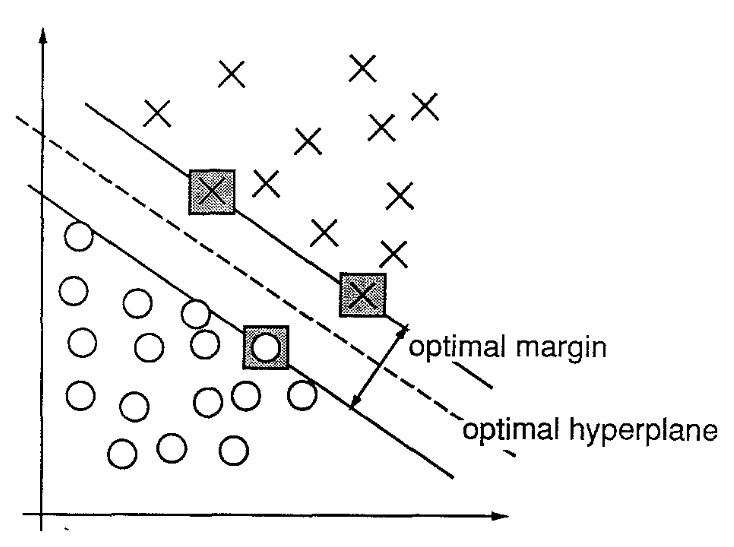
\includegraphics[width=0.6\linewidth]{./assets/images/svm-graph}
\end{figure}

\begin{textedited}
Além desta análise são utilizadas comparações de palavras dentro de um contexto previamente selecionado. Assim foi criado um \textit{cluster} de palavras comuns que facilita na identificação destas classes nos cabeçalhos analisados. Este \textit{cluster} basicamente é composto de:
\end{textedited}

\begin{itemize}
    \item Dicionário online padrão em sistemas Linux;
    \item 8441 nomes e 19613 sobrenomes;
    \item Sobrenomes chineses;
    \item Nome dos estados do Estados Unidos e das províncias canadenses;
    \item Nomes das cidades dos Estados Unidos;
    \item Nome dos países do mundo, de acordo com World Fact Book\footnote{Disponível em \url{https://www.cia.gov/library/publications/the-world-factbook/index.html}};
    \item Nome dos meses e suas respectivas abreviações.
\end{itemize}

Para cada uma das classes analisadas são feitas correlações com o tipo de dado esperado, de maneira a permitir que endereços de e-mail, por exemplo, sejam extraídos com base em expressões regulares utilizadas em linguagens de programação.

\begin{textnew}
Support Vector Machine é uma técnica conhecida principalmente por sua boa performance e habilidade para com grandes quantidades de dados, sendo por isso considerada uma boa solução para problemas de classificação. Por essa característica sua principal funcionalidade é baseada em opções, e a que mais se assemelha com a análise realizada é então classificada. Por isso Han \cite{Han-SVM} decidiu utilizar este mesmo conceito de comparação para ser então aplicado na extração de dados, de modo a confrontar e comparar classes de metadados, a fim de identificá-los e diferenciá-los.

Han também encontrou alguns desafios na diferenciação de campos, como é o caso dos múltiplos autores. Em alguns casos a diferenciação de autores, que fazem do mesmo campo, poderiam estar até em linhas ou grupos diferentes. Para isso foram utilizados alguns elementos para representar a separação dos nomes (\textit{chunks}), como pontuações e a palavra ''and''. Desta forma, os autores eram extraídos seguindo este padrão estipulado.

O resultado obtido pela utilização de SVM como técnica de extração de metadados foi bem relevante. O autor realizou uma comparação com a aplicação da técnica de Hidden Markov Models (HMM) - detalhada na \autoref{sssec:hmm} - onde a SVM se mostrou mais eficaz na precisão da extração para algumas classes específicas, como é o caso dos títulos, autores e endereços, por exemplo. Para outras classes a utilização da técnica de HMM ainda demonstrou ser mais eficiente na extração de metadados.

\end{textnew}

% Han também utiliza dicionários para facilitar na extração das informações

%Para o caso de extração de metadados em artigos científicos utilizando \textit{Support Vector Machines} \cite{Han-SVM} as tags de Seymore et al. \cite{Seymore-HMM-IE} são utilizadas para representação destas classes.

%Deste modo, com base nestas classes são definidas características de suas classes vizinhas, como por exemplo, elementos que ficam perto de outros elementos, que possuem uma sequência lógica geral de exibição. Com base nestas informações, que são feita classe por classe, estes padrões vão sendo encaixados a cada linha do cabeçalho analisado, permitindo que os metadados sejam extraídos com uma grande precisão.

% Parei a revisão aqui em 17/03/2015 23:22

\subsubsection{Hidden Markov Models (HMM)}
\label{sssec:hmm}

A teoria básica de Markov foi conhecida próximo dos anos 80 por engenheiros e matemáticos com grande aplicação inicialmente em processamento da fala, mas com vasta amplitude em outras áreas onde a descoberta de padrões pode ser aplicada \cite{Rabiner-HMM}.

O processo é baseado na identificação de modelos observáveis que representem e caracterizem a ocorrências de símbolos, ou seja, padrões, em determinados estados. Se um sinal foi observado ele pode ser utilizado para futuras referências, de acordo com o padrão. 

Um exemplo prático citado por Rabiner e Juang \cite{Rabiner-HMM} é o caso de uso do jogo  \textit{Cara e Coroa}. Toma-se um observador em um quarto fechado com uma cortina totalmente fechada para outro cômodo. Este observador não consegue ver nada que acontece no outro cômodo, onde está uma outra pessoa jogando uma moeda pra cima, relatando sempre o resultado obtido (cara ou coroa). Neste caso o problema é construir um modelo Hidden Markov Model (HMM) para explicar ao observador a sequência dos resultados obtidos. 

Neste exemplo, o primeiro caso é baseado tanto no estado de cada resultado (cara ou coroa) e em probabilidades matemáticas de ocorrência destes estados, neste caso, 0.5, ou seja, dois estados. Assim desenha-se modelos onde os estados são representados com base nas inúmeras possibilidades existentes, levando inclusive em consideração a sequência dos últimos acontecimentos. \begin{textnew}Outra possibilidade seria a existência de duas moedas, o que daria ainda dois estados existentes, mas não em função da probabilidade de sair cara ou coroa, mas sim por serem consideradas duas moedas ''justas'', o que daria também uma probabilidade de 0.5 pra cada.

Neste último exemplo o grande detalhe do modelo é que este é oculto (\textit{hidden}). Isso se deve ao fato de os dois estados, representados pelas duas moedas, serem totalmente independentes, o que não permite identificar qual moeda é a ''justa'' e então informar ao observador o resultado daquela rodada.

Por esta alteração de resultados e probabilidades, o fator decisivo na criação de cada modelo é a definição do número de estados que ele terá. Além disso, outro ponto que determina o sucesso do método é a utilização de um resultado anterior - \textit{training data set} -, ou seja, uma memória, um conjunto de informações pré-identificadas que permitiriam ainda à associação dos estados e ocorrência dos símbolos \cite{Rabiner-HMM}.

Um HMM pode ser formado por um conjunto de elementos, que formarão toda a teoria e aplicação dos algoritmos dentro do processo:

\begin{enumerate}
    \item Um número \texttt{N} de estados, onde \texttt{N} é um inteiro finito;
    \item Um intervalo temporal \texttt{t}, que determina a entrada em um novo estado, através de uma transição de probabilidade entre eles, levando em consideração sempre o estado anterior;
    \item Após cada transição o observador registra um \texttt{símbolo} de acordo com a distribuição de probabilidade, que por sua vez depende do estado atual do modelo.
\end{enumerate}

A utilização dos resultados passados - \textit{training data set} - é muito importante para uma boa definição de um HMM, visto que permite adaptar os parâmetros do modelo para aquele conjunto de dados passados, que por sua vez fazem parte de um padrão já identificado.

Seguindo este padrão o HMM pode ser utilizado, por exemplo, para reconhecimento de palavras isoladas que, juntamente com a utilização de um vocabulário de palavras permite a criação de modelos de reconhecimento. Cada palavra deste vocabulário seria um modelo HMM, permitindo que a palavra escolhida fosse a pertencente ao modelo com maior probabilidade.

\end{textnew}

Já no âmbito da extração da informação, o HMM pode ser aplicado conforme é apresentado por Seymore et al. \cite{Seymore-HMM-IE}, onde um modelo construído manualmente contendo múltiplos estados por campos (título, autor, etc), pode ser mais eficiente do que um modelo com um estado por campo. 


\begin{figure}
    \centering
    \caption{Exemplo de modelo HMM, onde X são os estados, Y as observações possíveis, A as probabilidades de mudança de estado e B as saídas das probabilidades.}
    \label{fig:hmm-states}
    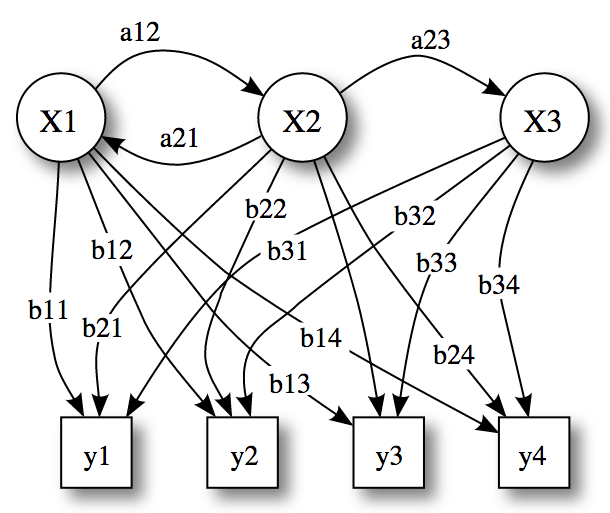
\includegraphics[width=0.7\linewidth]{./assets/images/hmm-states}
\end{figure}

\begin{textedited}
Um dos pontos positivos deste modelo é que por serem baseados em estatística eles são muito bem empregados em problemas de linguagem natural, aliando os resultados positivos à excelente performance computacional. Como desvantagem deste método podemos citar o fato de, por ser baseado em estatística, uma grande quantidade prévia de dados deve ser utilizada a título de treino para se obter padrões significativos para então ser aplicados de maneira final na criação do modelo.
\end{textedited}

Deste modo, para extração dos metadados, o HMM pode ser utilizado aplicando um marcador (\textit{label}) em cada palavra do cabeçalho de um documento (artigo científico), relacionando cada palavra a uma classe, como título, autor, etc. \begin{textnew}Assim, uma opção seria a criação de um modelo com \texttt{N} estados, onde cada estado corresponderia a uma classe que se deseja extrair - por exemplo o título do documento. Porém, no caso da existência de sequências ocultas (\textit{hidden sequences}) - o que alteraria a seleção do estado seguinte - a utilização de vários estados para cada classe traria resultados melhores \cite{Seymore-HMM-IE}.

% begin Seymore-HMM-IE

Para isso seria necessário entender melhor a estrutura do modelo de acordo com dados de treino (\textit{training data}), utilizando-se então de múltiplos estados para cada classe, o que traria resultados melhores. Deste modo, este \textit{training data} permitiria a construção de um modelo chamado \textit{maximally-specific model}. Neste modelo, cada palavra do \textit{training data} seria associada com seu próprio estado, com transição para o estado correspondente à palavra seguinte \cite{Seymore-HMM-IE}.

Este modelo - segundo os autores - poderia ser usado como o ponto de partida de uma variedade de técnicas para junção de estados (\textit{state merging techniques}). Desta forma os autores propõe duas formas de junção de estados que permita a construção deste \textit{maximally-specific model}:

\begin{enumerate}

\item \textit{\textbf{Neighbor-merging:}} combina todos os estados que compartilham transições e possuem o mesmo nome de classe. Por exemplo, uma sequência de estados correspondentes ao título seriam juntados em apenas um estado. Assim, vários estados vizinhos com os mesmos nomes de classes seriam juntados em apenas um.

\item \textit{\textbf{V-merging:}} combina quaisquer dois estados que possuem o mesmo nome de classe e compartilham transições ''de'' ou ''para'' um estado comum. Desde modo, ao invés de começar no estado inicial e decidir para qual estado correspondente ao título será feita a transição, esta técnica juntaria os estados ''filhos'' em um único estado, de maneira que somente uma transição do estado inicial para o estado de título iria existir. Desta forma, esta técnica poderia ser utilizada como modelo diretamente para extração de dados, podendo também criar novas combinações de estados, implicando em uma futura melhora deste modelo.

\end{enumerate}

Como o objetivo de Seymore et al. é extrair informações relevantes de cabeçalho de artigos de Ciência da Computação, a área de análise nestes documentos se limita até o início da introdução, ou ao final da primeira página, o que ocorrer primeiro.

O resumo (\textit{abstract}) é extraído facilmente com a utilização de expressão regular. Algumas classes de palavras especiais são identificadas também através de expressão regular e transformadas em \textit{tags} ou \textit{tokens}, como \texttt{<EMAIL>} ou \texttt{<YEAR\_NUMBER>}, por exemplo. Em todos estes casos, todos os acentos e informações de novas linhas (\texttt{\\n}) são removidos do texto.

Os resultados apontam como muito positiva a utilização de HMM para a extração de dados em cabeçalhos de artigos científicos. A precisão encontrada no experimento foi de 92,9\% para todas as classes do cabeçalho e, mais especificamente, 97,2\% para a extração dos autores. Também como resultado pode-se afirmar que modelos HMM com mais de um estado por classe são mais eficientes do que os que utilizam apenas um estado para cada classe analisada \cite{Seymore-HMM-IE}.

% end Seymore-HMM-IE

Uma outra utilização de HMM na extração de informação é descrita por \cite{Zhang-HMM-IE}, onde é realizado um experimento de extração de informação utilizando um conjunto de dados semi-estruturados, em formato HTML, contendo informações sobre restaurantes da cidade de Los Angeles.

Neste caso são estipulados quatro estados para o modelo: \textit{Background}, \textit{Prefix}, \textit{Suffix} e \textit{Target}. O \textit{Target} é o estado responsável pela emissão do símbolo - chamado pelo autor de \textit{token} - para o ''campo-alvo''. O \textit{Preffix} e \textit{Suffix} são estados que emitem símbolos que aparecem respectivamente antes e depois deste campo-alvo. Todos os demais símbolos são emitidos no estado \textit{Background}. A relação entre os estados pode ser visualizada na \autoref{fig:zhang-hmm-ie}.

\begin{figure}
	\centering
	\caption{Estados utilizados por \cite{Zhang-HMM-IE} em seu modelo HMM.}
	\label{fig:zhang-hmm-ie}
	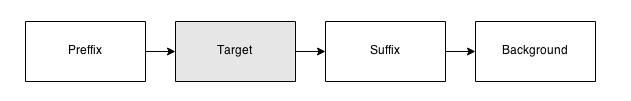
\includegraphics[width=0.8\linewidth]{./assets/images/zhang-hmm-ie}
\end{figure}

Os seguintes campos deveriam ser extraídos das informações dos restaurantes: \textit{restaurant name} (nome do restaurante), \textit{telephone number} (número de telefone), \textit{hours (horas)} e \textit{cuisine} (tipo de comida servida, como italiana, alemã, etc). Segundo Zhang \cite{Zhang-HMM-IE} os campos \textit{restaurant name} e \textit{telephone number} deveriam ser mais fáceis de serem obtidos, visto que o nome do restaurante geralmente se encontra em destaque, com alguma diferenciação visual. Já o telefone possui um formato numérico, que permite mais facilmente uma identificação de um padrão. O campo \textit{hours} também não foi complicado, embora se tenha uma variedade muito grande na disposição desta informação. Já o campo \textit{cousine} foi mais difícil de ser extraído, visto a diversidade que existe na forma de um restaurante especificar e/ou representar sua cozinha, tanto na utilização de palavras diferentes quanto na própria identificação do estilo do restaurante por si só.

Como resultados esperados, os campos \textit{restaurant name} e \textit{telephone number} obtiveram muito êxito em sua extração, com resultados realmente consideráveis. Já os campos \textit{hours} e \textit{cousine} não tiveram resultados muito satisfatórios, o que pode ser  explicado em função da característica dos HMMs de utilizar como modelo resultado de aprendizados anteriores, os \textit{training data set} ou simplesmente \textit{traning data}. Como nestes dois campos há uma grande possibilidade de representação diferente, os resultados não foram tão eficazes, o que poderia ser resolvido com uma alteração no modelo HMM que permitisse que as palavras identificadas como sendo do campo \textit{cousine} fossem capturadas de maneira mais proveitosa, que estão, neste modelo sugerido, isoladas no estado \textit{Background}.

Em função dos resultados obtidos, pode-se considerar a performance de HMM na extração de informação muito positiva, visto as possibilidades de variação do modelo, que permite um resultado mais acurado e próximo dos objetivos reais \cite{Zhang-HMM-IE}. Além disso, a utilização de resultados passados garante um aprendizado muito importante para que o modelo seja estabelecido, o que garante ainda mais um ganho de eficiência na aplicação desta técnica.

Além da utilização de HMM de forma natural, algumas variações de seu algoritmo são também citadas na literatura, como é o caso dos MEMMs (\textit{Maximum Entropy Markov Models}) \cite{maximum-entropy}. Nos MEMMs cada estado possui um modelo exponencial que utiliza as características de observação como entrada de dados (\textit{input}) \cite{Lafferty-CRF}. Estes modelos são baseados na técnica de HMM, se diferenciando na maneira como os estados se relacionam, bem como a relação entre suas transições, o que leva à citações de maneira independente por alguns autores, porém, com herança lógica dos conceitos de HMM.

\end{textnew}

\subsubsection{Word Clustering}
\label{sssec:word-clustering}

\begin{textnew}

Técnicas de classificação de texto geralmente utilizam palavras extraídas do texto como a principal fonte de recursos para a representação. Por outro lado, os \textit{clusters} de palavras tem sido uma proposta eficaz para a redução da dimensionalidade e da dispersão, melhorando assim a performance desta classificação \cite{Han-Giles-WC}.

Basicamente o conceito de \textit{clusters} compreende um conjunto de palavras formando um banco de dados de domínio (\textit{domain database}), aliado com um conjunto de propriedades ortográficas de demais palavras dentro daquele contexto específico. A utilização destes \textit{clusters} juntamente com outras técnicas tem mostrado um ganho de 6.6\% na performance de classificação de elementos de um cabeçalho de artigo científico, e ainda 8,4\% de ganho de performance para a extração da bibliografia destes documentos \cite{Han-Giles-WC}.

A utilização destes grupos de palavras demonstra uma relação entre palavras semelhantes dentro de um determinado contexto, permitindo que a extração dos metadados possa ocorrer de maneira mais eficaz, com resultados mais eficazes.

\end{textnew}


\begin{textedited}

Sendo assim, Han et al. apresentou uma ideia de um \textit{cluster} de palavras para promover a extração de metadados de artigos da área de Ciência da Computação, indo de maneira relativamente contrária às propostas tradicionais, que baseiam, geralmente, apenas na ocorrência e estatísticas de palavras isoladas dentro do texto original.

Han et al. agrupou bases de dados de domínios diversos incluindo também propriedades ortográficas de palavras, com base em um conhecimento prévio de classes específicas, como autor, título, etc. Deste modo, palavras encontradas nos documentos vão sendo comparadas com palavras deste \textit{cluster} construído, permitindo identificar, por grupos, características de metadados. Para cada classe cria-se um \textit{cluster}, com suas palavras e propriedades ortográficas específicas.

Como exemplo, a palavra ''Mary'' faz parte do contexto de ''nomes''. Portanto existe uma probabilidade maior de ela, juntamente com seu grupo de palavras ao redor, fazer parte da classe ''autor'', por exemplo. Esta lógica é apresentada para outras classes, como ''e-mail'' por exemplo, que pode ser identificado, em sua grande maioria, com a presença do caractere ''@'', o que levaria ao conceito de utilização de expressões regulares para encontrar padrões de ocorrências.

\end{textedited}

\begin{figure}
    \centering
    \caption{Workflow da extração de metadados usando \textit{cluster} de palavras}
    \label{fig:workflow-rule-based}
    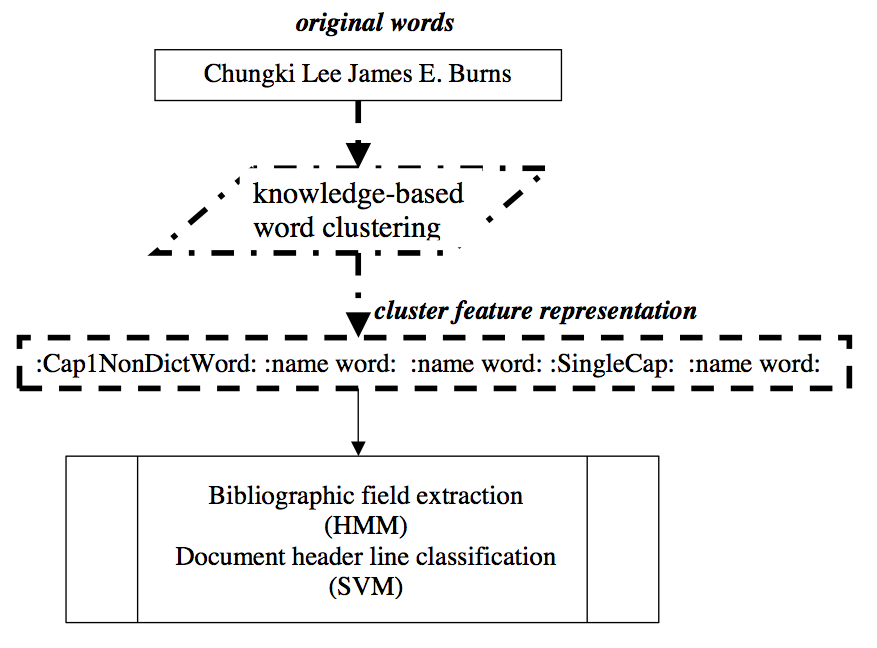
\includegraphics[width=0.7\linewidth]{./assets/images/workflow-rule-based}
\end{figure}

\begin{textnew}
A utilização de \textit{word clustering} tem demonstrado um custo computacional muito baixo, o que pode ser considerado uma vantagem sobre demais técnicas computacionais \cite{Han-Giles-WC}.
\end{textnew}

\begin{textedited}

Han et al. ainda utiliza da técnica  de SVM (\autoref{sssec:svm}) para classificação de linhas de um cabeçalho de um documento, tanto em função dos bons resultados obtidos quanto também pela boa performance apresentada. Deste modo, cada linha obtida se transforma em um vetor de palavras, que é comparado com seu respectivo \textit{cluster}, melhorando os resultados de classificação.

\end{textedited}

Além disso é utilizada também a técnica de HMM (\autoref{sssec:hmm}) para a extração das referências bibliográficas, observando sempre a ocorrência de padrões como título e autor para identificação dos mesmos em referências existentes no documento.

Basicamente a \textit{Rule-based Word Clustering} se resume em 3 (três) etapas. A primeira etapa se resume na construção das bases de dados, assim como \cite{Han-SVM}, onde foram utilizadas também como bases externas os nomes apresentados em seu \textit{cluster} (nomes de estados americanos, países, cidades, nomes de dicionários, nomes de pessoas, códigos postais, etc), de maneira a unir, não somente estas bases externas, mas também bases construídas dentro de um domínio específico, como palavras que pertencem a uma classe específica.

A segunda etapa é chamada de \textit{Cluster Design}. Nesta etapa é onde os \textit{clusters} são arquitetados, de maneira a contemplar também propriedades ortográficas das palavras, como se funcionasse de maneira geral como uma expressão regular de palavras, formando então este \textit{cluster} com base nas características apresentadas.

\begin{textedited}
Já a terceira etapa é chamada de \textit{Rule Design}, que resume-se basicamente na  combinação de palavras em diferentes domínios, na verificação ortográfica destas palavras e na classificação delas no seu \textit{cluster} correto. Por exemplo, nomes devem começar com a primeira letra maiúscula para então serem classificadas como pertencentes ao \textit{cluster} ''nomes''.
\end{textedited}

\begin{textnew}
Além disso, foi observada também a presença de certas palavras que faziam parte de diversos \textit{clusters} ao mesmo tempo, o que permitiu que elas fossem classificadas em seu próprio grupo de palavras, tornando-se então independentes.
\end{textnew}

\begin{textnew}
A representação através de \textit{clusters} utilizada por Han et al. \cite{Han-Giles-WC} conseguiu reduzir um texto original de 11.223 palavras em um \textit{cluster} de 588 elementos, permitindo ainda que ele fosse distribuído entre as classes distintas, o que tornou o processo muito menos trabalhoso mas, ao mesmo tempo, eficaz.
\end{textnew}

\begin{textedited}
Como resultado, a utilização desta técnica de clusterização permitiu um ganho considerável de performance, além de permitir uma precisão maior dos resultados, visto que eles são apresentados com base nestas bases focadas em um domínio específico, perfazendo um contexto mais definido e com resultados mais garantidos.

Por outro lado a utilização desta técnica possui uma falha na semântica dos dados. No momento da classificação das classes, na separação e criação dos \textit{clusters}, um dígito ou conjunto deles é substituído por \texttt{:number:}. Isso faz com que ele se torne apenas um número qualquer, sem um contexto específico, ou seja, pode ser tanto uma referência a alguma página do documento ou até mesmo um mês de um ano.

\end{textedited}


\subsubsection{Conditional Random Fields (CRFs)}
\label{sssec:crf}

% Falar sobre CRFs 

CRFs é um framework proposto por Lafferty et al. \cite{Lafferty-CRF} criado para construir modelos probabilísticos e dados marcados em sequência (\textit{label sequence data}), geralmente utilizados no reconhecimento de padrões e aprendizado de máquinas (\textit{machine learning}).

\begin{textnew}

Esta técnica oferece algumas vantagens ao se comparar com técnicas mais tradicionais, como HMM (\autoref{sssec:hmm}), se destacando a habilidade de diminuir pressupostos independentes feitas nestes modelos \cite{Lafferty-CRF}.

Modelos baseados em HMM possuem uma fraqueza, que é problema denominado \textit{bias problem}. As transições de um dado estado somente competem entre elas, e não com todas as transições presentes no modelo. Elas são feitas com base probabilística de acordo com o estado inicial e a sequência de observação (\textit{observation sequence}).

Desta forma, devido ao \textit{bias problem}, em um caso extremo, um estado que tiver como opção de transição somente um outro estado, pode simplesmente ignorar a sequência de observação, o que traria efeitos contrários aos objetivos do processo.

Laffarty et al. realiza comparações funcionais e práticas entre CRFs, HMM e MEMM (\textit{Maximum Entropy Markov Models}), uma variação da técnica de HMM, detalhada na \autoref{sssec:hmm}. A diferença crítica entre CRFs e MEMMs é que MEMM utiliza como probabilidade de ocorrência de um próximo estado modelos exponenciais para cada um deles, enquanto a técnica de CRF possui um modelo exponencial único para toda a sequência de \textit{labels}, com base na sequência de observação. Segundo Laffarty et al. \cite{Lafferty-CRF} pode pensar na CRF como um modelo de estado finito sem normalização das probabilidades de transição.

Uma das vantagens de se utilizar CRFs sobre HMM é que ela absorve todas as qualidades deste último, mas com a particularidade de resolver o \textit{bias problem}. Outra grande vantagem ao ser comparada com HMMs e MEMMs é que a CRF possui resultados melhores quando a distribuição dos dados possui grande dependência do modelo, o que geralmente ocorre em casos mais práticos.

Um exemplo para entender o \textit{bias problem} foi apresentado por Lafferty et al. \cite{Lafferty-CRF}. Ele propõe um modelo cujo objetivo é distinguir duas palavras: \texttt{rib} e \texttt{rob}, tendo como sequência de observação as letras \texttt{r i b}. O problema é identificado quando uma das duas palavras é mais comum no \textit{training set}, o que acarreta nas transições do estado inicial preferirem suas transições correspondentes, o que acarreta sempre na vitória da palavra relacionada aquele estado.

Visando a comprovação e reconhecimento da eficiência da técnica de CRF na extração de informação, foram aplicados dois tipos de experimentos:

\begin{enumerate}
    \item Verificação direta do \textit{bias problem};
    \item Geração de dados utilizando HMM aleatórios.
\end{enumerate}

Os resultados apontam que HMMs superam MEMMs em virtude do \textit{bias problem}. Por sua vez os CRFs superam os HMMs, sendo então considerada a CRF a melhor técnica a ser empregada com base no \textit{training set} utilizado \cite{Lafferty-CRF}. Outro ganho apresentado pode ser verificado ao agregar algumas características ortográficas à utilização de CRFs, aumentando o poder destes modelos condicionais.

De modo geral as CRFs utilizam a mesma lógica que modelos baseados em Markov (HMMs e MEMMs), se diferenciando nos aspectos probabilísticos para com as transições entre os estados, acarretando em resultados comparativos melhores. Por corresponder a uma ''máquina'' de estado finito, ela é muito aplicável para a função de classificação sequencial, o que permite que ainda seja treinada para se obter os melhores resultados probabilísticos \cite{Peng-CRF-IE}. Nas CRFs as transições de estado são também representadas como \emph{features} por alguns autores.

\end{textnew}

%Esta técnica é comparada e quase sempre utilizada juntamente com a HMM (Hidden Markov Models), de maneira a possuir algumas vantagens sobre esta última, como a habilidade de relacionar pressupostos independentes nos modelos, ou seja, relacionar observações e/ou interpretações.

Uma outra vantagem da técnia de CRFs - assim como dos modelos \emph{maximum entropy} - é que eles facilmente proporcionam o uso de características arbitrárias dos dados de entrada.

Os CRFs são utilizadas também em marcação e classificação de dados sequenciais, com uma ordem determinada, como linguagem natural, sequências biológicas (como os genes) ou estados computacionais.

% Falar sobre o uso de CRFs na extração de informação

Sua aplicação na extração de metadados foi apresentada por Peng et al. \cite{Peng-CRF-IE}, como uma maneira eficaz de extrair metadados em cabeçalhos e referências de artigos científicos. Deste modo, através da identificação destes padrões sequenciais pode-se determinar os tipos de dados existentes e então identificá-los, seguindo uma lógica/ordem pré-determinada.

\begin{textnew}
Peng et al. apresenta resultados desta extração utilizando Conditional Random Fields (CRF) e aponta também algumas questões acerca da utilização testa técnica para este tipo de atividade. Os autores comparam as CRFs com técnicas de HMM \autoref{sssec:hmm} e SVM \autoref{sssec:svm}, mencionando que a forma de trabalhar com CRF aponta parte das vantagens destas duas técnicas, destacando o a junção entre as sequências e características dependentes mas ao mesmo tempo arbitrárias. Ainda assim, a utilização de CRFs para a tarefa de extração de metadados possui melhoras, segundo os autores, dramáticas, ao se comparar com as demais técnicas de SVM e HMM.

Os autores definem quatro diferentes transições de estado para diferentes classes, em ordem diferente das técnicas derivadas de Markov (HMM):

\begin{enumerate}
    \item \emph{\textbf{First-order:}} os dados de entrada são examinados no contexto de somente um estado;
    \item \emph{\textbf{First-order + transitions:}} são adicionados alguns parâmetros correspondentes às transições;
    \item \emph{\textbf{Second-order:}} as entradas são examinadas no contexto dos estados atual e anterior;
    \item \emph{\textbf{Third-order:}} os dados de entrada são examinados no contexto do estado atual e de dois estados anteriores.
\end{enumerate}

Para a extração destes dados Peng et al. também considera como sendo o cabeçalho de um \emph{paper} como sendo a parte inicial do documento até o início da introdução, ou somente a primeira página, o que ocorrer primeiro. Além disso, os autores consideram como os campos a serem analisados os mesmos 15 (quinze) que foram definidos anteriormente por Seymore et al. \cite{Seymore-HMM-IE}.

Do \emph{dataset} para extração dos metadados de cabeçalhos utilizado foram analisados 935 (novecentos e trinta e cinco) documentos. Destes 500 (quinhentos) foram utilizados para compor o \emph{training set} e os outros 435 (quatrocentos e trinta e cinco) para fins de teste unicamente. Já do \emph{dataset} utilizado para extração das referências foram analisados 500 (quinheitos) documentos, dos quais 350 (trezentos e cinquenta) foram utilizados para \emph{training set} e os demais 150 (cento e cinquenta) também para testes.

Para os fins de resultados comparativos foram utilizadas três métricas:

\begin{enumerate}
    \item \emph{\textbf{Overall word accuracy:}} é uma métrica que utiliza a porcentagem de palavras das quais os nomes (\emph{labels}) previstos são exatamente seus valores reais. Esta métrica favorece aqueles campos que possuem muitas palavras, como por exemplo a introdução (\emph{abstract});
    \item \emph{\textbf{Average F-measure (F1):}} esta métrica é contada se baseia na exatidão das ocorrências, considerando tanto a precisão quanto a memória de todos os campos (\emph{fields}). Esta metrica favorece campos com poucas palavras, visto sua característica mais importante focar na exatidão dos resultados.
    \item \emph{\textbf{Whole instance accuracy:}} nesta métrica uma ''instância'' é considerada como sendo todo um cabeçalho ou referência, de maneira integral. Desta forma esta métrica utiliza da porcentagem de instâncias das quais cada palavra é corretamente associada.
\end{enumerate}

Conforme pode-se observar na \autoref{tab:crf-results-headers} e \autoref{tab:crf-results-references} a utilização de CRFs para extração de metadados - tanto de cabeçalhos como das referências - teve resultados melhores do que a utilização de HMM (\autoref{sssec:hmm}), aumentando a performance em praticamente todos os campos, chegando a uma precisão de 98,3\% (\emph{overall accuracy}).

Pode observar também que a utilização de modelos HMM para precisão de palavras (campos com poucas palavras, onde a precisão é muito mais importante) é, de modo geral, pior que quando utiliza-se SVMs (coluna F1 da \autoref{tab:crf-results-headers}). Por outro lado, no campo \emph{abstract} HHM possui performance bem melhor que quando utilizado SVM (98\% contra 93,8\%).

\begin{table}
    \caption{Resultados de extração para CRFs após análise do \emph{dataset} com cabeçalhos \cite{Peng-CRF-IE}.}
    \begin{center}
        \begin{tabular}{|c|c|c|c|c|c|c|} \hline             
             & \multicolumn{2}{c|}{HMM} & \multicolumn{2}{c|}{CRF} & \multicolumn{2}{c|}{SVM} \\  \hline 
            Overall acc. & \multicolumn{2}{c|}{93.1\%} & \multicolumn{2}{c|}{\textbf{98.3\%}} & \multicolumn{2}{c|}{92.9\%} \\ \hline
            Instance acc. & \multicolumn{2}{c|}{4.13\%} & \multicolumn{2}{c|}{\textbf{73.3\%}} & \multicolumn{2}{c|}{-} \\ \hline \hline
             & acc. & F1 & acc. & F1 & acc. & F1 \\ \hline
            Title & 98.2 & 82.2 & 99.7 & \textbf{97.1} & 98.9 & 96.5 \\ \hline
            Author & 98.7 & 81.0 & 99.8 & \textbf{97.5} & 99.3 & 97.2 \\ \hline
            Affiliation & 98.3 & 85.1 & 99.7 & \textbf{97.0} & 98.1 & 93.8 \\ \hline
            Address & 99.1 & 84.8 & 99.7 & \textbf{95.8} & 99.1 & 94.7 \\ \hline
            Note & 97.8 & 81.4 & 98.8 & \textbf{91.2} & 95.5 & 81.6 \\ \hline
            Email & 99.9 & 92.5 & 99.9 & \textbf{95.3} & 99.6 & 91.7 \\ \hline
            Date & 99.8 & 80.6 & 99.9 & \textbf{95.0} & 99.7 & 90.2 \\ \hline
            Abstract & 97.1 & 98.0 & 99.6 & \textbf{99.7} & 97.5 & 93.8 \\ \hline
            Phone & 99.8 & 53.8 & 99.9 & \textbf{97.9} & 99.9 & 92.4 \\ \hline
            Keyword & 98.7 & 40.6 & 99.7 & \textbf{88.8} & 99.2 & 88.5 \\ \hline
            Web & 99.9 & 68.6 & 99.9 & \textbf{94.1} & 99.9 & 92.4 \\ \hline
            Degree & 99.5 & 68.8 & 99.8 & \textbf{84.9} & 99.5 & 70.1 \\ \hline
            Pubnum & 99.8 & 64.2 & 99.9 & 86.6 & 99.9 & \textbf{89.2} \\ \hline
            \hline
            Average F1 & & 75.6 & & \textbf{93.9} & & 89.7 \\ \hline
        \end{tabular}
    \end{center}
    \label{tab:crf-results-headers}
\end{table}

\begin{table}
    \caption{Resultados de extração para CRFs após análise do \emph{dataset} com referências \cite{Peng-CRF-IE}.}
    \begin{center}
        \begin{tabular}{|c|c|c|c|c|} \hline             
             & \multicolumn{2}{c|}{HMM} & \multicolumn{2}{c|}{CRF} \\  \hline 
            Overall acc. & \multicolumn{2}{c|}{85.1\%} & \multicolumn{2}{c|}{\textbf{95.37\%}} \\ \hline 
            Instance acc. & \multicolumn{2}{c|}{10\%} & \multicolumn{2}{c|}{\textbf{77.33\%}} \\ \hline \hline
             & acc. & F1 & acc. & F1 \\ \hline 
            Author & 96.8 & 92.7 & 99.9 & \textbf{99.4} \\ \hline 
            Booktitle & 94.4 & 0.85 & 97.7 & \textbf{93.7} \\ \hline 
            Date & 99.7 & 96.9 & 99.8 & \textbf{98.9} \\ \hline 
            Editor & 98.9 & 70.8 & 99.5 & \textbf{87.7} \\ \hline 
            Institution & 98.5 & 72.3 & 99.7 & \textbf{94.0} \\ \hline 
            Journal & 96.6 & 67.7 & 99.1 & \textbf{91.3} \\ \hline 
            Location & 99.1 & 81.8 & 99.3 & \textbf{87.2} \\ \hline 
            Note & 99.2 & 50.9 & 99.7 & \textbf{80.8} \\ \hline
            Pages & 98.1 & 72.9 & 99.9 & \textbf{98.6} \\ \hline
            Publisher & 99.4 & \textbf{79.2} & 99.4 & 76.1 \\ \hline
            Tech & 98.8 & 74.9 & 99.4 & \textbf{86.7} \\ \hline
            Title & 92.2 & 87.2 & 98.9 & \textbf{98.3} \\ \hline
            Volume & 98.6 & 75.8 & 99.9 & \textbf{97.8} \\ \hline
            \hline
            Average F1 & & 77.6\% & & \textbf{91.5\%} \\
            \hline
        \end{tabular}
    \end{center}
    \label{tab:crf-results-references}
\end{table}

\end{textnew}

\begin{textedited}
Com base nos resultados apresentados pode-se considerar que a trabalho de \cite{Peng-CRF-IE} contribuiu para o estado da arte, melhorando a performance na extração de metadados em artigos científicos. Assim, a utilização de CRFs mostra-se muito eficaz por reduzir consideravelmente os erros encontrados, aumentando o sucesso da aplicação desta técnica neste contexto.
\end{textedited}




\section{Revisão de Estado da Arte na Extração de Metadados}
\label{sec:revision}

\begin{textnew}

% Falar aqui sobre os estudos de comparações de Granitizer

Técnicas de \emph{machine learning} não são novas, porém suas aplicações vão muito mais além do que se podia imaginar. As técnicas então utilizadas para apenas classificação de palavras e processamento de linguagem natural foram sendo utilizadas em diversas outras áreas, resolvendo problemas distintos e inovando em soluções, como é o caso da extração de informação.

O aperfeiçoamento da aplicação destas técnicas para a área de \emph{information extraction} acarretou em um resultado muito positivo, melhorando cada dia mais a precisão dos resultados obtidos. Assim, algoritmos foram/são alterados e otimizados visando obter maiores performances e resultados melhores.

Pode-se perceber que cada técnica de classificação e/ou extração de informação possui suas particularidades e características técnicas diferentes. Assim, nota-se que cada uma possui uma melhor aplicação para extração de determinado campo, ou conjunto deles. Pequenas modificações são necessárias para que todo o contexto de um artigo científico seja mapeado com sucesso, sendo às vezes necessária a utilização de diversas técnicas em um único projeto.

Para isso, diversas comparações destas técnicas foram feitas. Algumas, inclusive já mencionadas ao longo deste trabalho, foram feitas no surgimento de uma nova técnica, onde esta era comparada com técnicas anteriores, a fim de comprovar sua aplicabilidade e aumento de performance. Porém, este tipo de comparação torna-se tendencioso, visto que os campos analisados, bem como os \emph{datasets} utilizados, tendenciam para resultados positivos da nova técnica apresentada. Além disso, geralmente os \emph{datasets} utilizados são focados em documentos da área de Ciência da Computação, e tendem a seguir um padrão visual já estipulado pelos grandes eventos da área.

Em função deste problema alguns autores realizam comparações de técnicas, isoladamente ou com utilização de ferramentas, para analisar um grupo de documentos reais, objetivando um resultado mais próximo da realidade e, consequentemente, mais passível de erros.

Granitzer et al. \cite{Granitzer-2012-LayoutBased} comparam o uso de Conditional Random Fields (\autoref{sssec:crf})) e Support Vector Machines (\autoref{sssec:svm})) na extração de metadados em artigos científicos, utilizando para tal \emph{datasets} multidisciplinares, como \emph{Mendeley} e \emph{e-Prints}, que fazem parte de um grupo social de \emph{datasets}, permitindo a contribuição global, unindo pesquisadores de diversas áreas do conhecimento, construindo um repositório diversificado e recheado de novos desafios reais.

Em função da existências destes repositórios a informação fica cada vez mais descentralizada e, portanto, é necessária cada vez mais mecanismos inteligentes para garantir a alta qualidade dos metadados extraídos e armazenados de cada documento \cite{Granitzer-2012-LayoutBased}. A combinação destes mecanismos com pós-processamento inteligente contribui para o processo, elevando a qualidade do resultado final encontrado.

% CiteSeer e Mendeley utilizam SVMs. Granitzer 2012

Visando um reconhecimento maior dos resultados obtidos Granitzer et al. realizam comparações dos resultados obtidos com a aplicação de três ferramentas: ParsCit (\autoref{ssec:parscit})), Mendeley Desktop (\autoref{ssec:mendeley})) e sua própria ferramenta baseada em CRFs, no qual se referem como Layout-based CRF.

Este trabalho \cite{Granitzer-2012-LayoutBased} é uma continuação do trabalho anteriormente realizado \cite{Granitzer-2012-Crowdsourced}, onde as ferramentas Mendeley Desktop (\autoref{ssec:mendeley}) e ParsCit (\autoref{ssec:parscit})) foram comparadas, utilizando, porém, um \emph{dataset} menor. Desta vez foi incluída a técnica de Conditional Random Fields (CRF) na comparação, que de acordo com a literatura mencionada neste trabalho, possui resultados melhores do que com a utilização da técnica Hidden Markov Models (HMMs - \autoref{sssec:hmm}).

Foram analisadas 20.672 publicações do \emph{dataset} Mendeley, abrangendo diversas áreas do conhecimento como ciência de modo geral, ciência da computação, biomedicina e física. Já no \emph{dataset} e-Prints foram analisadas 2.452 publicações de áreas como física, medicina e diversas outras pertencentes ao IEEE, ligadas geralmente à área de computação.

Foi relatado que umas etapas principais para um processamento eficaz e uma extração mais precisa é o pós-processamento. A aplicação de diversas análise, inclusive matemáticas, nos resultados extraídos garante um conjunto de dados de saída muito melhor e mais acurado. Segundo Granitzer et al. \cite{Granitzer-2012-LayoutBased} estas tarefas são mais de responsabilidade do setor de engenharia, onde diversos detalhes devem ser observados e diversos algoritmos devem ser aplicados.

De modo geral, os resultados obtidos pelas ferramentas Mendeley e ParsCit foram considerados ruins para os grupos pertencentes à área médica \cite{Granitzer-2012-LayoutBased}. Porém estes resultados poderiam ser melhorados com um novo treino dos dados (\emph{training set}), com aplicações específicas para aquela área do conhecimento, no caso, medicina. Outro ponto interessante observado foi que a extração dos títulos ocorreram mais facilmente do que a extração dos autores, que possui sua performance muito variada em função da técnica que é utilizada.

Para os outros grupos, os resultados foram bem positivos, observando uma pequena diferença entre os números obtidos com as ferramentas Mendeley e ParsCit, que foram muito superiores aos resultados da implementação CRF dos autores. Isso se deve ao fato das duas ferramentas anteriores utilizarem de pós-processamento dos dados, o que garantiu aos resultados obtidos uma precisão muito maior \cite{Granitzer-2012-LayoutBased}.

De acordo com Gratnizer et al., mesmo a técnica de CRF possuindo melhores modelos de extração de informação, foi-se observada que a técnica de SVM utilizada pelo Mendeley Desktop supera a CRF no que tange extração de metadados \cite{Granitzer-2012-LayoutBased}.

A ferramenta ParsCit de modo geral não teve resultados melhores do que o modelo do Mendeley Desktop. Para a área de Ciência da Computação, mais especificamente na base de dados do IEEE, ambas as ferramentas tiveram excelentes resultados. Já na base de dados da ACM o Mendeley obteve melhores resultados do que o ParsCit \cite{Granitzer-2012-LayoutBased}.

\end{textnew}

\section{Técnicas de Algoritmos}
\label{sec:algorithms-tecniques}

\comment{Este tópico foi sugestão do Prof. Renato. Qual o conteúdo deve ser colocado neste tópico?}

\section{Ambientes de Extração de Metadados}
\label{sec:environments}

Alguns projetos baseiam sua extração em padrões pré-definidos de maneira a identificar dados relevantes dentro de uma região específica, facilitando a procura e consequentemente aumentando a velocidade no resultado. 

Estes projetos geralmente permitem uma variedade muito grande de layouts, embora nem todos já estejam previamente definidos. Geralmente novos layouts são inseridos em novas versões ou até mesmo por contribuições das mais diversas, como é o caso dos projetos de código livre, os chamados projetos \textit{open source}.

Abaixo segue uma relação dos principais projetos relacionados à área de extração de metadados de artigos científicos, com informações sobre seu funcionamento e algoritmos que são utilizados.

\subsection{Cermine}
\label{ssec:cermine}

% CERMINE

Um destes projetos é o recente CERMINE \cite{cermine}, uma biblioteca \textit{open source} desenvolvida na linguagem de programação Java que permite que sejam extraídos os metadados de artigos científicos em formato digital PDF, oferecendo ainda a possibilidade de cruzamento de dados por meio de referências e títulos, permitindo assim identificar citações bem como a relevância de um determinado documento.

O CERMINE ainda possui um mecanismo de aprendizagem da própria máquina, permitindo que na medida que dados forem sendo alterados ele consiga absorver os detalhes e permitir assim uma mudança de sua maneira de extrair os dados. Deste modo ele permite que seja adaptado para novos padrões de layouts, o que permite de maneira geral que uma grande gama de modelos seja então abrangida. 

Seu grande diferencial em comparação com as demais técnicas é que ele não somente extrai os metadados de um artigo, mas sim analisa todo o seu conteúdo, incluindo citações a outros artigos, que podem ser facilmente cruzados por meio de informações como título e autor(es).

Seu mecanismo considera somente arquivos PDF com texto gerado de maneira pura, sem a utilização de imagens. Basicamente ele considera regiões, linhas e páginas como pontos estratégicos para a extração de informações. As bases destas regiões possuem padrões que são utilizados juntamente com técnicas de SVM \cite{Han-SVM}. Com base nisso ele condensa um layout onde as informações geralmente estão dispostas, permitindo assim que em um determinado local do arquivo esteja, provavelmente, o título e o nome dos autores. 

Com estas regiões definidas o CERMINE extrai as informações com base em padrões preestabelecidos, de maneira a gerar então sua saída para os metadados e sua saída para as referências encontradas. A saída trabalhada pelo projeto é no formato XML, permitindo assim que possa ser compartilhado com outros sistemas por possuir uma leitura semântica e ao mesmo tempo fácil de ser interpretada pelas linguagens de máquinas. A \autoref{fig:cermine-workflow} demonstra como o processo de extração do CERMINE funciona.

\begin{figure}
    \centering
    \caption{CERMINE Extraction Workflow}
    \label{fig:cermine-workflow}
    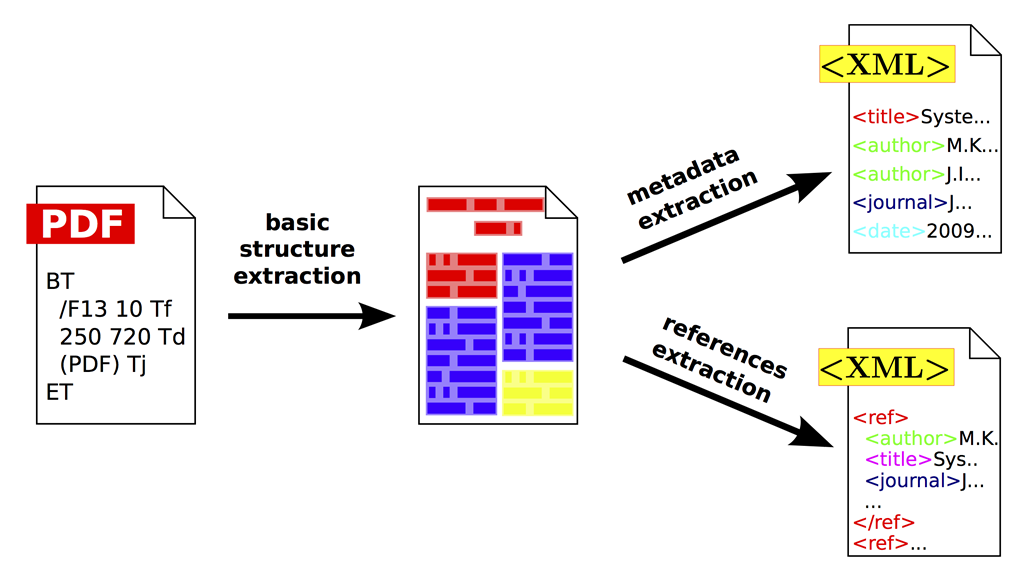
\includegraphics[width=0.7\linewidth]{./assets/images/cermine}
\end{figure}

Com o mapeamento definido ele identifica regiões de acordo com seu conteúdo, as quais ele chama de \textit{zones}. Esta regiões são determinadas a fim de extrair as informações relevantes para cada uma, de maneira a separar, por exemplo, a área destina aos metadados do arquivo. O CERMINE divide estas \textit{zones} da seguinte maneira:

\begin{itemize}
    \item \textbf{Metadata:} É a região mais ao alto do documento, onde obtém os metadados, que seriam o resumo, \textit{bib\_info}, tipo, título, afiliação, autores, datas, editores e palavras-chaves.
    \item \textbf{References:} Região responsável por identificas detalhes de referências que foram utilizadas no artigo, como título e autores, por exemplo
    \item \textbf{Body:} O texto geral do artigo, incluindo equações, imagens e tabelas.
    \item \textbf{Other:} Outros detalhes menos significantes semanticamente, como número das páginas, dentro outros.
\end{itemize}

A extração das referências abrange também seus próprios metadados. Tanto no texto corrido (\textit{Body}) quanto na lista de referências do artigo o \textit{parser} do CERMINE analisa linha a linha, permitindo uma extração de dados mais eficaz. Das referências são extraídos os seguintes dados: autor, título, nome do \textit{journal}, volume, \textit{issue}, páginas, \textit{publisher}, localização e o ano.

\subsection{TeamBeam}
\label{ssec:teambeam}

Outros projeto de destaque é o TeamBeam \cite{teambeam}, cuja base ideológica possui objetivos bem sociais, de contribuir com o compartilhamento de conhecimento. Basicamente o objetivo do projeto é extrair metadados de artigos científicos, porém focado apenas nestes, de maneira a extrair título, nome do \textit{journal}, resumo e informações sobre os autores, como nome, endereço de e-mail e afiliações.

O projeto também é de código livre (\textit{open source}) e é baseado na extração de pequenos blocos de texto. A manipulação dos arquivos PDF são feitas pela biblioteca PDFBox \footnote{Biblioteca de manipulação de arquivos PDF mantida pela Fundação Apache. Disponível em \url{https://pdfbox.apache.org/}}, que fornece meios eficazes de extrair textos com base nas regiões desejadas.

O algoritmo do TeamBeam utiliza o algoritmo de \textit{Maximum Entropy} \cite{maximum-entropy}, que utiliza basicamente de tarefas de classificação sequencial como ferramenta principal para obtenção de padrões. A base deste algoritmo está na utilização de CRFs \cite{Lafferty-CRF}, principalmente no que diz respeito à extração dos metadados \cite{Peng-CRF-IE}.

O processo de extração é feito basicamente em duas etapas. A primeira é a etapa de classificação de blocos de texto (\textit{text block classification}), onde geralmente já é possível obter algum dado concreto de resultado. Neste etapa o objetivo é associar certos blocos de texto a um dos seguintes marcadores: \textit{Title Block}; \textit{Sub-Title Block}; \textit{Journal Block}; \textit{Abstract Block}; \textit{Author Block}; \textit{E-Mail Block}; \textit{Affiliation Block}; \textit{Author-Mixed Block}; e \textit{Other Block}.

Dependendo do layout do artigo alguns metadados podem vir divididos em blocos de texto diferentes, necessitando de um processamento posterior, como é o caso, geralmente, dos blocos com informações sobre os autores. Neste caso também é realizada a etapa de classificação de token (\textit{token classification}), que se resume na classificação de palavras individualmente de acordo com um dos seguintes marcadores: \textit{Given Name}; \textit{Middle Name}; \textit{Surname}; \textit{Index}; \textit{Separator}; \textit{E-Mail}; \textit{Affiliation-Start}; \textit{Affiliation}; e \textit{Other}.

Kern et al. defendem a ideia dos excelentes resultados do TeamBeam ao ser comparado com outros projetos. Este fato é dado em virtude das características que são levadas em consideração no processamento do algoritmo, utilizando de dicionários, informações de layout e modelo de linguagem.

\subsubsection{Resultados Comparativos}
\label{sssec:teambeam-comparative}

A fim de analisar os resultados obtidos com a aplicação das técnicas descritas no TeamBeam, os autores comparam as técnicas utilizadas com outras técnicas de outras ferramentas, que utilizam processos diferentes de análises.

Para fins de comparação de resultados, os autores citam as técnicas ParsCit (\autoref{ssec:parscit}), Layout-CRFs (\autoref{ssec:layout-crfs}) e Mendeley Desktop (\autoref{ssec:mendeley}). Como conclusão ele compara estas três técnicas separadamente, por não abrangerem todos os detalhes que o TeamBeam possui, o que tornaria a comparação desleal.

Assim, ele chega à conclusão que em virtude das diferentes formas de processamento dos dados feitas por cada umas das ferramentas, chega-se a resultados mais precisos para cada campo extraído. Por exemplo, o Layout-CRF's (\autoref{ssec:layout-crfs}) é mais abrangente e mais assertivo para extração de títulos, por ser baseado em CRF. Já as ferramentas baseadas em dicionário apresentam melhores resultados para extração de autores, visto se basearem em \textit{data-sets\footnote{Bases de dados com nomes dos autores mais citados e outras informações já catalogadas que são armazenadas para consulta pública.}} já consolidados.

\subsection{Mendeley}
\label{ssec:mendeley}

\begin{textnew}

Mendeley é um dos projetos mais complexos e completos que existem na atualidade. Além de uma poderosa ferramenta na extração de metadados o projeto se transformou em uma plataforma completa para pesquisadores. Sua pesquisa se iniciou em novembro de 2007 por três estudantes alemães de doutorado, tendo sua primeira versão lançada em agosto de 2008. Em 2013 o projeto foi vendido para uma empresa, que passou a liderar o processo de criação e desenvolvimento. Atualmente o Mendeley é um projeto amplo, porém estritamente comercial, que possui uma plataforma de pesquisa e gestão de documentos como seu principal produto ofertado.

Os serviços oferecidos possuem modalidades grátis e paga, de acordo com a necessidade do usuário. Assim como o CiteULike \autoref{ssec:citeulike} o projeto se tornou referência no meio acadêmico, sendo utilizado e comentado por diversos pesquisadores. Em virtude de seu objetivo comercial a ferramenta não possui código aberto, o que não permite seu uso sem ser através do serviço oferecido pela empresa, através da Internet.

A ferramenta pode ser utilizada via Web, como aplicativo \emph{desktop}, para \emph{tablets} ou \emph{smartphones}. Visto seu aspecto social e suas inúmeras funcionalidades o projeto se tornou uma rede social acadêmica, tanto do ponto de vista de organização de documentos até mesmo para interação entre pesquisadores. A ferramente permite que usuários façam \emph{upload} de artigos em formato PDF para que sejam armazenados em sua biblioteca pessoal. Estes arquivos são analisados e seus metadados são extraídos e enviados para os servidores centrais da ferramenta.

Além de organizar sua biblioteca pessoal é possível também fazer anotações em documentos, destacar partes de texto, exportar citações, gerenciar documentos e compartilhar informações com outros pesquisadores, o que torna a plataforma extremamente completa e funcional.

A pesquisa iniciada pelos três estudantes de doutorado levou em consideração técnicas de \emph{machine learning} e \emph{metadata extraction}, como SVM, por exemplo \cite{Granitzer-2012-LayoutBased}. A ferramenta utiliza um modelo de SVM de dois estágios (\emph{two-stages SVM}) \cite{Han-SVM} no que tange a extração dos metadados, obtendo uma grande exatidão dos resultados.

Pela sua complexidade e por abranger uma gama de funcionalidades muito grande, s serviço foi comparado à rede Last.FM \cite{Mendeley-LastFM}. Assim como a rede social de música o Mendeley permite que o usuário organize sua biblioteca digital de pesquisa de maneira bem eficaz, podendo compartilhar, distribuir e realizar diversas outras funções, assim como é possível na plataforma musical Last.FM.

Por ser um serviço a bastante tempo no mercado o Mendeley funciona também como um grande \emph{dataset}, permitindo que parte de sua coleção de artigos seja utilizada para fins de pesquisa, assim como ocorre com o CiteULike \autoref{ssec:citeulike}, por exemplo. Isso facilita muito a pesquisa pois permite que uma quantidade muito grande de documentos sejam analisados de maneira semi-estruturada, facilitando a descoberta de novos conhecimentos nesta área.

Após a venda da plataforma o projeto teve seu foco muito mais voltado ao comercial, ao contrário do que era anteriormente. A utilização de seus dados ficou restrita e a geração de receita se transformou no principal objetivo da companhia, o que trouxe algumas desvantagens para a pesquisa livre como um todo.

Algumas das funcionalidades do Mendeley:

\begin{itemize}
    \item Multiplataforma, podendo funcionar tanto na Web como em Windows, Mac, Linux, iPhone e iPad;
    \item Extração de metadados de artigos em formato PDF (ponto de pesquisa deste trabalho);
    \item Centralização de sua biblioteca digital, sendo a mesma disponibilizada em qualquer plataforma, pois fica disponível na nuvem (\emph{cloud computing});
    \item Visualizador de PDF embutido, o que permite marcações em texto e inclusão de notas personalizadas;
    \item Pesquisa completa da base de dados dos artigos existentes;
    \item Inclusão de \emph{tags} nos documentos, permitindo uma categorização dos mesmos dentro da biblioteca pessoal de cada usuário;
    \item Permite que citações e bibliografias sejam exportas em formato Microsoft Word, LibreOffice e \LaTeX;
    \item Criação de grupos públicos e privados entre pesquisadores, permitindo compartilhamento de conteúdo entre os usuários;
    \item É uma Rede Social completa, permitindo \emph{posts}, comentários, páginas de perfil, etc;
    \item Provém uma série de estatísticas com base nos documentos pertencentes à sua biblioteca digital.
\end{itemize}

% Mendeley usa two-stages SVM method \cite{Han-SVM} e \cite{Granitzer-2012-LayoutBased}

Embora o sucesso do projeto seja muito grande e suas funcionalidades permitem uma série de funções a serem utilizadas pelos pesquisadores, em virtude do foco deste trabalho, o Mendeley se torna uma ferramenta pouco útil, visto que não possui o seu código aberto e não permite que seu código seja instalado em outras máquinas para que sua funcionalidade de extração de metadados seja testada. Mesmo assim, o projeto é bastante promissor e garante uma gama de funções que todo pesquisador necessita, além de organizar de maneira bem eficaz os artigos e demais documentos que fazem parte de um bom trabalho de pesquisa.

\end{textnew}

\subsection{CiteULike}
\label{ssec:citeulike}

\begin{textnew}

Uma outra ferramenta de destaque é o CiteULike \cite{citeulike} e pode ser acessada em \url{http://citeulike.org}. Ela é uma fusão de dois serviços: um serviço de \emph{bookmarking} via Internet, bem como também um sistema de gestão de referências bibliográficas. A união destas duas funcionalidades permite um compartilhamento muito grande de conhecimento entre pesquisadores, de modo a promover uma disseminação de informação com o envio de links contendo \emph{papers} de pesquisa. 

O projeto foi criado em 2004 por Richard Cameron, mas em 2006 a empresa Oversity Ltd. assumiu seu controle e manutenção \cite{CiteULike-FAQ}. O CiteULike pode ser acessado através de um navegador e fica disponível na Internet, de fácil acesso. O projeto ainda encontra-se ativo e em constante evolução, tanto por parte da equipe que o mantém, como por parte de seus usuários.

O projeto é livre desde seu lançamento e não tem nenhum custo para seus usuários. Seu objetivo inicial surgiu de um problema para busca de material bibliográfico. Deste modo o CiteULike foi criado para remover este espaço vazio entre pesquisadores, além de permitir que eles compartilhem bibliografias de maneira simplificada, podendo inclusive contribuir para grupos de pesquisa, por exemplo.

Um dos detalhes desta ferramenta é que ela funciona com base em fontes externas de dados. Quando um usuário encontra na Internet um artigo que lhe é interessante ele pode adicioná-lo à sua lista pessoal (\emph{bookmarking}). Assim, o CiteULike automaticamente visita este endereço informado e realiza uma extração de dados dos detalhes das citações do artigo, salvando o link para este \emph{paper} em sua base de dados \cite{citeulike}. Além disso, ele permite que os metadados deste artigo também sejam extraídos, como título, autores, \emph{journal name}, número de páginas, etc.

Como se pode ver, o CiteULike preserva a informação livre. Ele somente coleta \emph{papers} que já estão disponíveis na Internet, com base em um link fornecido por um usuário seu. Outro ponto de interesse é que a ferramenta também analisa informações de citação para que possa criar um link reverso para os \emph{papers} já analisados. Deste modo, de posse de um link para um determinado artigo o CiteULike consegue analisar quais outros artigos este artigos cita, permitindo criar uma rede de citações entre documentos, o que facilita a disseminação de conhecimento e permite que pesquisadores distintos possam usufruir deste conjunto de informações previamente analisadas.

Outro detalhe importante é o fato do projeto ser ao mesmo tempo um serviço social. Além do armazenamento destes artigos em forma de links, ao adicionar um artigo em sua lista pessoal, o usuário também pode associar \emph{tags} àquele artigo. Isso permite uma categorização muito particular e ainda permite que artigos sejam procurados bem facilmente com bases nestas \emph{tags} fornecidas. De certa forma, outros pesquisadores podem se beneficiar destas informações, pois elas funcionam como uma folksonomia específica para aquele determinado domínio, que pode ser de interesse de outros pesquisadores também. Outro detalhe importante de destaque do ponto social da ferramenta é que ela permite um sistema de votação nos artigos. Cada artigo pode ser votado por usuários, de maneira a criar-se um ranking de artigos mais interessantes, tendo um local de destaque na página inicial da ferramenta.

Um grande detalhe do CiteULike é que ele permite que suas informações sejam utilizadas para análise de dados futuros, permitindo assim uma evolução da área de \emph{machine learning} e \emph{metadada extraction}. Como o CiteULike cria uma rede de artigos, ao mesmo tempo ele possui um banco de dados muito rico, que pode se utilizado como um \emph{dataset}, visto suas informações semi-estruturadas. Inclusive os autores citam o fato de já existirem diversos projetos independentes atualmente que utilizam o \emph{dataset} do CiteULike para realizar suas análises \cite{citeulike}. Atualmente na base de dados do CiteULike podemos encontrar mais de 7.900.000 (sete milhões e novecentos mil) artigos.

Como o banco de dados do CiteULike é criado de forma estruturada a disseminação de conhecimento entre os pesquisadores é facilmente realizada. De posse do link para um determinado artigo a ferramenta possui todos os detalhes deste documento, como título, autores, etc. Assim permite-se uma pesquisa muito rica em um conjunto de metadados previamente extraídos, criando então uma rede de distribuição de artigos, contribuindo para a comunicação entre pesquisadores de modo geral.

O projeto cumpriu basicamente duas regras:

\begin{enumerate}
    \item Ele criou um modelo para coleta de informações que é de fácil entendimento para o usuário final, extraindo metadados relevantes que permitem criar automaticamente uma rede de conteúdo, sem deixar de apontar para o artigo em seu site original;
    \item Ele mudou a maneira tradicional de descobrir e compartilhar informação, visto que a ferramenta permite que usuários acessem suas listas pessoais entre si, disseminando conhecimento com base em um conhecimento já pré-definido por um pesquisador.
\end{enumerate}

Outro detalhe que permite um uso diferenciado do projeto é a formação de grupos de pesquisa. Com base em interesses similares no histórico de pesquisa, o CiteULike permite que pesquisadores sejam ligados globalmente, compartilhando de temas semelhantes e compartilhando informações entre eles de maneira eficaz e direta.

Tecnicamente o CiteULike foi criado utilizando como banco de dados o PostgreSQL\footnote{Sistema de Banco de Dados relacional com tradição e excelente performance. Sua página inicial é \url{http://www.postgresql.org}.}, Tcl\footnote{Linguagem de programação de scripts muito utilizada em ambientes Linux. Pode ser acessada em \url{http://www.tcl.tk}.} como linguagem de programação e ainda utilizando Memcached\footnote{Sistema de cacheamento baseado em memória, que permite um ganho excelente de performance em ambientes Web, sendo uma das mais utilizadas nos dias atuais. Detalhes em \url{http://memcached.org}.} para criação de cache dos dados armazenados, o que aumentou (e muito) a performance da ferramenta. Seus servidores são baseados em Linux e backups são feitos de 15 em 15 minutos \cite{citeulike}.

Com base nesta quantidade de detalhes e vantagens o CiteULike se tornou um ponto de referência para catalogação e organização de artigos científicos, permitindo a contribuição entre pesquisadores e formando então uma rede de contribuição que favorece a disseminação da pesquisa ao redor do mundo.

\end{textnew}


\subsection{CiteSeer}
\label{ssec:citeseer}

Um dos projetos mais específicos encontrados é o CiteSeer \cite{citeseer}. Seu objetivo não é apenas extrair dados em artigos, mas sim também analisar citações de outros documentos no conteúdo textual encontrado. Assim, ele é capaz de identificar quais documentos são citados, quantas vezes são citados e onde são citados, se assemelhando muito ao processo de citação natural. O CiteSeer foi criado pelos pesquisadores Lee Giles, Kurt Bollacker e Steve Lawrence em 1997 e utiliza modelos SVM para extração de metadados com bastante eficácia \cite{Granitzer-2012-LayoutBased}.

Desta forma, com estas informações identificadas, ele consegue criar um \textit{ranking} dos documentos citados, incluindo seus autores e \textit{journals}, criando a partir de um documento fonte todo um conjunto de relações com outros documentos de uma maneira estatística bem eficaz.

Os indexes de citações (\textit{citation indexes}), que são utilizados no projeto, foram originalmente criados para a recuperação de informação, porém sua utilidade é tamanha que permite que citações sejam indexadas de maneira eficaz, permitindo inclusive que referências de documentos em idiomas diferentes sejam identificadas. Desta maneira, essa técnica pode ser utilizadas de diversas formas, não somente na identificação de citações propriamente ditas, mas envolvendo um conjunto de informações eficazes, como inclusive identificar a reputação de um determinado artigo científico no meio em que se encontra, simplesmente analisando onde é referência em relação ao número de vezes em que é citado.

Uma proposta interessante em que se baseia o CiteSeer é a de Cameron \cite{cameron}. Seu objetivo é de formar uma Base de Citações Universal, onde todos os artigos estariam ligados entre si, independente de qualquer fator externo como idioma, por exemplo. A diferença entre esta proposta e o trabalho realizado com o CiteSeer é que este último permite que os documentos sejam analisados sem nenhum esforço extra, ou seja, sem a intervenção dos autores dos documentos, como é proposto por Cameron. Neste caso, os documentos seriam analisados de maneira automática, diminuindo o tempo necessário para o relacionamento de todos eles e aumentando a eficácia e eficiência do processo.

O funcionamento do CiteSeer é relativamente simples, porém o trabalho realizado por detrás do processo envolve muito estudo e dedicação. Basicamente ele é capaz de fazer o \textit{download} de \textit{papers} utilizando a Internet, convertê-los em texto e realizar a análise de todas as suas citações. Este resultado é armazenado em um banco de dados para consultas e relacionamentos futuros. Um dos pontos interessantes desta análise é que como ela é feita com base em referência textual, identificado origem e destino, ela pode ser facilmente aplicada tanto no sentido natural de leitura (um artigo cita outros) quanto no sentido inverso (um artigo é citado por outros). 

O projeto também possui suas desvantagens, como por exemplo, a não cobertura de alguns \textit{journals} importantes, indexando todos seus documentos online e de maneira automática. Além disso o projeto original não é capaz de identificar mais de um autor nos documentos, sendo a identificação apenas pelo campo autor, tendo ele apenas um ou mais de um pesquisador envolvido.

Basicamente o projeto analisa o documento em partes:

\begin{itemize}
    \item \textbf{URL:} a URL onde o documento foi obtido;
    \item \textbf{Cabeçalho:} o bloco de título e autor do documento;
    \item \textbf{Resumo:} o bloco de resumo do documento;
    \item \textbf{Introdução:} a introdução do texto do documento;
    \item \textbf{Citações:} a lista de referências a outros documentos citadas no decorrer do texto;
    \item \textbf{Contexto de citação:} o contexto no qual um documento cita outro;
    \item \textbf{Texto completo:} o texto completo do documento e suas respectivas citações como um todo.
\end{itemize}

Um dos detalhes importantes do projeto é a identificação das \textit{tags} de citações, que são basicamente as representações visuais quando um outro documento é referenciado, como por exemplo: [4], [Giles997] e ''Marr 1982''. Estes pequenos pedaços de textos que permitem ao CiteSeer identificar a relação (e em que momento do texto) entre documentos, permitindo assim que suas análises sejam realizadas de maneira eficaz.

Uma das dificuldades relatadas durante o desenvolvimento do projeto é a identificação de artigos iguais com formas de escrita e informações divergentes. Alguns artigos podem vir com autores com sobrenomes utilizando abreviação, ou até mesmo em ordem diferente. A fim de aumentar esta identificação alguns passos a mais são realizados, como a conversão para caixa baixa todas as letras, remoção de hifens e das próprias \textit{tags} de citação, expansão de abreviaturas e remoção de algumas palavras externas como ''\textit{volume}'', ''\textit{pages}'' e ''\textit{number}'' por exemplo.

O CiteSeer é um projeto bem maduro e abrangente. Após cerca de 18 (dezoito) anos desde sua criação ele ainda se encontra ativo na Internet, abrangendo cada vez mais documentos e aprimorando cada vez mais suas técnicas de identificação de documentos.

\subsection{ParsCit}
\label{ssec:parscit}

\begin{textedited}
Assim como o CiteSeer o ParsCit é um projeto baseado na identificação de citação de documentos. Porém eles utiliza um modelo de CRF \textit{(Conditional Random Fields)} para identificar sequências nas referências bibliográficas, utilizando uma implementação desta técnica chamada CRF++ \cite{Councill-Giles-2008-ParsCit}.
\end{textedited}

O projeto encontra-se ainda ativo e possui atuais contribuições de desenvolvedores ao longo do mundo. Desenvolvido na linguagem de programação \textit{Perl}, o projeto pode ser executado tanto na forma de um \textit{web service\footnote{É a disponibilização de algum serviço na Internet permitindo que outros projetos consultem suas informações e as obtém de maneira simplicada.}} quanto de maneira \textit{standalone}, com execução do código direto quando necessário, dentro do servidor.

Um detalhe bastante interessante do projeto é a descrição de seu processamento antes e depois da análise do documento, que os autores chamam de \textit{Pre-Processing Steps} e \textit{Post-Processing Steps}.

Inicialmente o processamento inicia buscando certos \textit{tokens} que podem estar ligados a alguma referência, seja em formato numérico, seja na citação dos nomes dos autores nos mais diversos formatos. Com essa referência coletada o próximo passo é buscar dentro do artigo onde ela está localizada, com base em um conjunto de heurísticas previamente definidas. Para isso é necessária a conversão total do conteúdo do artigo para o formato texto, que deve estar codificado em UTF-8\footnote{Formato de exibição de caracteres que englobam os formatos mais utilizados no mundo, com acentuação e caracteres especiais.} \cite{Councill-Giles-2008-ParsCit}.

Desta forma a fase de pré-processamento se inicia com esta analise puramente textual, em busca de padrões comuns que podem ter sido utilizados para representações de referências à artigos científicos. Com os resultados coletados um modelo CRF é então aplicado aos dados encontrados para processamento futuro.

Com este modelo CRF definido algumas etapas são aplicadas a fim de normalizar os dados encontrados. Nomes de autores podem estar escritos de maneira diferente, com abreviações em nomes de maneira diferente, dependendo do modo como as referências foram escritas no artigo analisado.

Esta análise posterior dos nomes dos autores é feita com base na inspeção de cada palavra individualmente, respeitando então um padrão de normalização definido, sempre com as iniciais dos nomes seguidas do sobrenome escrito normalmente.

A utilização deste projeto é feita de maneira muito simples, podendo ser executado por linha de comando, o que facilitam os testes e a extração de dados. Os resultados obtidos desta análise é então exibido (ou gravado em arquivo) em formato XML, que permite utilização posterior em qualquer tecnologia. Como informado anteriormente os resultados também podem ser coletados em formato de \textit{Web Service}, mas para os fins desta pesquisa apenas sua execução em linha de comando é suficiente.

\subsubsection{Resultados Comparativos}
\label{sssec:parscit-comparative}

Visando comparar os resultados obtidos com alguns projetos em que o ParsCit foi baseado, os autores realizam comparações com os resultados obtidos pelo processo descrito por Peng \cite{Peng-CRF-IE}, onde de maneira geral obteve uma melhora na extração e comparação das referências em torno de 5\% (precisão de 0.91 passou para 0.95), demonstrando a eficácia do projeto (detalhes na \autoref{tab:parscit-results}).

\begin{table}
    \caption{Resultados comparativos entre ParsCit e Peng \cite{Peng-CRF-IE}}
    \begin{center}
        \begin{tabular}{|c|c|c|c|c|c|}
            \hline 
            \multirow{2}{*}{Field} & \multicolumn{3}{c|}{ParsCit} & \multicolumn{2}{c|}{Peng} \\
            \cline{2-6}
             & Precision & Recall & F1 & Acc. & F1 \\ 
            \hline
            Author & 98.7 & 99.3 & .99 & 99.9 & .99 \\
            Booktitle & 92.7 & 94.2 & .93 & 97.7 & .94 \\
            Date & 100 & 98.4 & .99 & 99.8 & .99 \\
            Editor & 92.0 & 81.0 & .86 & 99.5 & .88 \\
            Institution & 90.9 & 87.9 & .89 & 99.7 & .94 \\
            Journal & 90.8 & 91.2 & .91 & 99.1 & .91 \\
            Location & 95.6 & 90.0 & .93 & 99.3 & .87 \\
            Note & 74.2 & 59.0 & .65 & 99.7 & .81 \\
            Pages & 97.7 & 98.4 & .98 & 99.9 & .99  \\
            Publisher & 95.2 & 88.7 & .92 & 99.4 & .76 \\
            Tech & 94.0 & 79.6 & .86 & 99.4 & .87 \\
            Title & 96.0 & 98.4 & .97 & 98.9 & .98 \\
            Volume & 97.3 & 95.5 & .96 & 99.9 & .98 \\
            \hline
            Average & 95.7 & 95.7 & .95 & – & .91 \\
            \hline
        \end{tabular}
    \end{center}
    \label{tab:parscit-results}
\end{table}

Visando também analisar outros projetos a mesma comparação de resultados foi feita com o projeto CiteSeer \cite{citeseer}, onde o aumento da qualidade dos dados extraídos foi de aproximadamente 19\% levando em consideração algumas limitações do CiteSeer que não são compreendidas como no ParsCit.

% Falar de cada trabalho encontrado com base nos eventos

	% Falar um resumo
	% Diferencial do projeto
	% Se está ativo ou não
	
% \comment{Seria necessário falar também do Weka (\textit{The open-source machine learning framework})? Até que ponto ele seria relevante para a pesquisa em si? Neste caso tenho medo de fugir muito do escopo e detalhar demais técnicas.}

\subsection{Outras Ferramentas e Projetos}
\label{ssec:other-tools}

\begin{textnew}

Além das ferramentas apresentadas diversas outras apresentam características semelhantes, porém com pouca participação de mercado ou com foco em funcionalidades que não são objetos de estudo deste trabalho, como por exemplo, somente o foco no armazenamento e gestão dos artigos científicos. Alguns destes projetos que pode-se citar são:

\begin{itemize}
    \item \textbf{Zotero:} Seu objetivo é servir como um repositório centralizado onde os artigos ficam armazenados, permitindo que as referências sejam exportadas para diversos formatos. Disponível em \url{https://www.zotero.org}.
    \item \textbf{Citavi:} Permite que você organize artigos científicos de maneira bem estruturada, permitindo inclusive contribuição através de formação de times de pesquisadores. Também permite exportação de suas referências para diversos outros formatos. Disponível em \url{http://www.citavi.com/}.
    \item \textbf{BibDesk:} Exclusivo para usuários Mac/Apple. É um \emph{software} final que permite que usuários organizem seus artigos, simplificando todo o processo de exportação dos formatos de referências. É focado para usuários \LaTeX. Disponível em \url{http://bibdesk.sourceforge.net}.
    \item \textbf{Docear:} Permite que usuários organizem suas bibliotecas digitais de artigos científicos, permitindo também compartilhar informações com outros usuários. Possui versões para Windows, Linux e Mac. Disponível em \url{https://www.docear.org/}.
    \item \textbf{Qiqqa:} Permite que além de organizar os usuários façam gestão das referências de seus artigos, que ficam armazenados também em \emph{cloud computing}. Possui versões Windows e Android. Disponível em \url{http://www.qiqqa.com/}.
    \item \textbf{Papers:} Aplicativo disponível para Windows, Mac, iPhone e iPad que permite que usuários gerenciem e pesquisem artigos científicos. Possui um banco de dados próprio e é oferecido apenas em versão paga. Disponível em \url{http://www.papersapp.com/}.
    \item \textbf{JabRef:} Muito parecido com a ferramenta \emph{BibDesk}, visto que organizar artigos e referências focados em usuários \LaTeX. Possui versões para Windows, Linux e Mac. Uma de suas vantagens é possuir uma interface muito simplificada, facilitando a utilização pelos usuários. Disponível em \url{http://jabref.sourceforge.net/}.
    \item \textbf{EndNote:} Além de permitir a organização muito bem estruturada de artigos científicos ele é também uma ferramenta de pesquisa, permitindo também exportar seu catálogo de referências para os mais diversos formatos. Possui versões para Windows e Mac, podendo ser acessado também através da Web. Disponível em \url{http://endnote.com/}.
\end{itemize}

\end{textnew}

